\chapter{Introduction}\label{ch:introduction}

One of the research topics in Computer Vision that has become of interest in recent years is the detection of abnormal activities in surveillance videos. 

Nowadays, more than ever, public safety has become a great concern. Therefore, public spaces need to be monitored for any individual(s) that might be acting out of the ordinary with the intent of doing harm to someone else or even with the intent of stealing something.

Thus, the need for automated surveillance systems has increased, with the objective of assisting security officers in performing their job more efficiently.

Computer Vision algorithms can be used to detect and track moving targets in a video feed and extract features that allow a system to analyze and classify such targets as performing abnormal or suspicious behaviors and send an alert to security officers.

The classification of such behaviors is not linear and so research needs to be done in order to develop a system that can accurately detect different types of suspicious behaviors.

\section{How are Anomalous and Suspicious behavior different?}

\begin{figure}
  \centering
  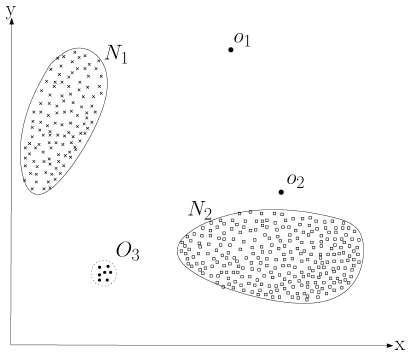
\includegraphics[width=0.5\textwidth]{figures/Anomalies_in_2D_data.png}
  \caption{An example of anomalies in two-dimensional data set\cite{n23}.}
  \label{fig:AnomaliesExample1}
\end{figure}

Anomalous behavior or anomalies are patterns in data that are different from predefined normal behaviors (normal model). Figure \ref{fig:AnomaliesExample1} shows an example of anomalies in a two-dimensional data set. There are two normal regions \(N_{1}\) and \(N_{2}\), all points that are lying outside those regions are considered anomalies. Those patterns might be a result of malicious activity, system failure or noise in the data. Therefore, the relevance of anomalies to real life is a key feature in anomaly detection\cite{n24}.

Novelty detection is also closely related to anomaly detection \cite{n16,n17}. Unlike anomaly detection, novelty detection is concerned with finding newly developed or previously unknown patterns that a system was not aware of ,or failed to recognise during training. The main difference between the two is that novel patterns are typically later incorporated in the normal model.

While anomalous behavior can be described as behavior which differs from the expected, suspicious behavior is not that simple to model. Suspicious behavior is detected through subjective interpretation and presents a challenge even for human observers. Often the ability to predict how a situation will develop is helping in detecting suspicious behavior. Human observers rely on their experience often described as 'sixth sense' or 'gut feeling', to correctly detect suspicious behavior \cite{n18}. Context is another very important part of suspicious behavior detection. Behavior that is considered normal can become suspicious in a different context. Because of that, the normal behavior model needs to be updated over time as the context changes. This makes labeling data for training nearly impossible and it is also impossible to generate a data set capturing all possible human behaviors\cite{n24}.


\section{Challenges}

Since anomalies are considered deviations from the normal model, detecting them should be straight forward. One solution would be to define a normal region and all observations outside that region are abnormal. However, several issues arise when trying to implement that approach.

- It is very difficult to define a normal region, that correctly represents every possible normal behavior. In addition, the separation between normal and abnormal is not always clearly defined.

- When the anomalies are caused by malicious actions, those actions are usually made to appear normal.

- The normal behavior is prone to change over time. A model which is currently a good representation of normal behavior might not be sufficient in the future.

- It is hard to find labeled data for training models.

- Detecting suspicious behavior is very subjective and depends on how actions are interpreted.

- Given behavior might be considered suspicious in one context but normal in another and because the context changes the system needs to account for that.

Because of those challenges it is not easy to create a general solution for detecting suspicious behavior. Instead most solutions are focused on very specific formulation of the problem.


\section{Problem Statement}
To Do



\section{Related Work}

The detection of suspicious behavior by automatic systems has raised a lot of interest in recent years. To be able to accurately detect suspicious behavior a system needs to have an understanding of general human behavior but also needs to understand the context in which this behavior is presenting itself.

Wiliem et al. \cite{n1} propose a context-based system for detecting suspicious behavior. This work considers that a system like this needs to have three main components. Firstly, it needs to continuously extract and learn contextual and human behavioral information from the video stream. Hence, a context space model is introduced in which the systems designers select important information that can describe a context but also allows the system to distinguish between two different instances of contexts. Secondly, it exploits contextual information in making decisions by introducing the use of a data stream clustering algorithm that enables the system to continuously update its knowledge from the data. This algorithm is capable of retrieving knowledge learned from a specific context. Lastly, the system incorporates an inference algorithm that combines contextual information and the system's knowledge to make decisions. The system also incorporates human observers' input in the decision making.

To test the system, experiments were done using the CAVIAR data set \cite{n19} and a private data set. The experiments showed that the system made accurate detections due to using previously acquired knowledge relevant to the context. The system was even able to detect unexpected events.

A lot of researchers resort to machine learning for detecting suspicious behavior which mostly relies on having reliable standard data sets for training and testing which, sometimes, might be hard to acquire. To overcome this issue Elhamod and Levine \cite{n2} propose a semantics-based solution which is based on human reasoning and logic. This solution elaborates a mathematical framework based on abstract descriptions shown by Fuentes and Velastin \cite{n3} for detecting suspicious behavior and also builds up on previous work by the same authors \cite{n4}.

Their proposed framework tracks people and luggage in a scene. Behaviors and events happening in a scene are semantically recognized by extracting object and inter-object motion features. The context of the investigation was the detection of suspicious behavior in public transport areas.

While earlier articles focus on detecting only one type of behavior \cite{n5,n6}, this work analyzes different types of behavior relevant to the context such us: abandoned and stolen objects, fighting, fainting and loitering.

Detected objects in a scene are classified as being animate (e.g. people) or inanimate (e.g. luggage) which are the semantic entities associated with the events described. The extracted features are divided into single-object and inter-object. The single-object features include position, speed, direction and merged (a Boolean that specifies whether an object is merged with another or not), while distance, alignment and speed difference are the inter-object features. The method follows the concept presented by Bird et al. \cite{n6} which uses motion features to classify objects into four categories: \textit{unknown U}, \textit{abandoned object O}, \textit{person P}, and \textit{still person SP}. The motion features are calculated and recorded in historical records and behaviors are semantically defined and detected by checking the records against predefined rules and conditions.

Public data sets such as BEHAVE \cite{n20}, CAVIAR (PETS 2004) \cite{n21} and PETS 2006 \cite{n22} were used to test this framework. The results showed that the framework successfully detects all of the events discussed.

Methods for detecting suspicious behavior are usually developed for specific types of behaviors. To improve the accuracy of the system many methods require complex feature extraction algorithms that do not allow for the systems to be used in real-time. To solve this, Mu et al. \cite{n7} present a fast method for detecting suspicious behavior such as wandering, trailing, chasing and falling down. The proposed method is based on the extraction of motion vectors from a video stream to obtain the necessary features to classify behaviors in a video.

7-D features \(\{\theta, V, \sigma_{\theta}, \sigma_{V}, E_{\theta}, E_{V}, Inter_{Dj}\} \) are extracted from a frame to describe each target detected. \(\theta\) and V represent the average direction and velocity of the target; \(\sigma_{\theta}\) and \(\sigma_{V}\) represent the direction variance and the velocity variance; \(E_{\theta}\) and \(E_{V}\) represent entropy of direction and velocity; \(Inter_{Dj}\) is the interesting degree of inter-frame \(Inter_{D}\). The direction, velocity and inter-frame difference proved to be the most important features. A Support Vector Machine (SVM) is used to learn and classify the input videos.

The results from the experiments are compared with those in \cite{n8,n9,n10,n11} and this method, in the majority of aspects, shows significant improvements when compared with the other methods.

In order to increase the efficacy of a video-surveillance control center for a shopping mall, in comparison with traditional methods, Arroyo et al. \cite{n12} investigated the detection of suspicious behavior in shopping malls. The analyzed risk situations in this context were a shop entry or exit of people, loitering events that can lead to theft and unattended cash desk situations.

The proposed approach employs an innovative tracking method that manages occlusions based on SVM kernels to compute distances between appearance features such as GCH (Global Color Histogram), LBP (Local Binary Pattern) and HOG (Histogram of Oriented Gradients). With these features, color, texture and gradient information are combined to obtain a robust visual description of people in videos.

The analysis of people's entrance or exit from the shops is important in the detection of crowded situations when a lot of people enter a shop at the same time or when people run away when exiting. For this, the line of the entrance to the shop is manually placed and the directions of people passing by are analyzed.

For loitering detection, risk zones are specified and loitering is detected whenever someone is in an area for a period of time longer than a defined threshold.

Unattended cash desks are a risky situation because someone might try to steal money from the cash register if no one is looking. Hence, an alarm is given if a person is detected loitering around an unattended cash desk.

To evaluate the performance of their system, the publicly available CAVIAR data set was used for testing occlusion situations and the system showed to be slightly superior to multiple others state-of-the-art methods \cite{n13,n14,n15}. The system was also tested on a private data set and it was concluded that it could detect suspicious behaviors in the intended context.

State-of-the-art approaches need to take into consideration the context in which they want to detect suspicious behavior in order to accurately do so. There is still a lot of research that can be done to unveil new ways and approaches on how to implement even more efficient systems.


\section{Organization}
To Do


